\begin{frame}{Introduction -> 2 Frequency dependent fitness}

    \begin{itemize1}    
        \item Game theory.
        \item $OncoSimulR$ is intended to create a model taking into account the interactions between different subpopulations (individual or common benefit).
        \item Frequency dependent selection: the fitness of a subpopulation will depend on the relative abundance of the different subpopulations.
        \item With $OncoSimulR$ -> fitness of each subpopulation as an arbitrary function of the genetic interactions between multiple genes.       
    \end{itemize1}
    
\end{frame}

\begin{frame}{Introduction -> Effects on fitness}

    \begin{itemize1}
        \item $allFitnessEffects$ function:
        \begin{itemize2}
            \item $genoFitness$ = dataframe
            \begin{itemize3}
                \item First column: genotypes.
                \item Second column: expressions for the functions that relate fitness to frequencies of other genotypes.
            \end{itemize3}
            \item $frequencyDependentFitness$ = TRUE
            \item $frequencyType$ = “rel” or $frequencyType$ = “abs”
            \item $spPopSizes$
        \end{itemize2}        
    \end{itemize1}

\end{frame}

\begin{frame}{Introduction -> Assess fitness}

    \begin{itemize1}
        \item $evalGenotype$ function:
        \begin{itemize2}
            \item $fitnessEffects$ = $allFitnessEffects$ object
            \item $genotype$
        \end{itemize2}
        \item $evalAllGenotypes$ function:
        \begin{itemize2}
            \item $fitnessEffects$ = $allFitnessEffects$ object
        \end{itemize2}
    \end{itemize1}
    
\end{frame}

\begin{frame}{Introduction -> Perform simulations}

    \begin{itemize1}
        \item $oncoSimulIndiv$ and $oncoSimulPop$ functions.
    \end{itemize1}
    \begin{columns}
        \begin{column}{0.5\textwidth}
            \begin{figure}[t]
                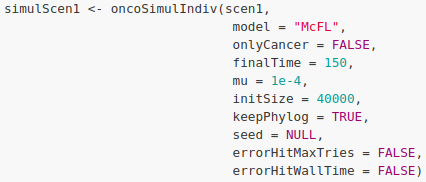
\includegraphics[width=0.9\linewidth]{img/oncoSimulIndiv.png}
            \end{figure}
        \end{column}
        \begin{column}{0.5\textwidth}
            \begin{figure}[t]
                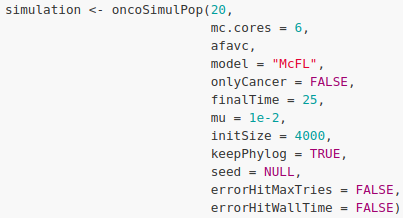
\includegraphics[width=0.9\linewidth]{img/oncoSimulPop.png}
            \end{figure}
        \end{column}
    \end{columns}
\end{frame}
    
\end{frame}
